Science and technology are constantly reshaping the agricultural landscape. Industrial revolutions of the 19th and 20th centuries replaced handheld tools and horse-driven plows with gasoline engines and chemical fertilizers. In the 21st century, agriculture is witnessing another major paradigm shift with unprecedented automation in every aspect of food production and farm management. Now, there exists commercial tools for automating recurring farming tasks such as seeding~\cite{tanimura_plant_2019}, weeding~\cite{weeding}, irrigation~\cite{shock2002automation}, fertilization~\cite{fertilizing}, application of pesticides~\cite{anderson2013robotic}, harvesting~\cite{gamaya_gamaya_2019}, and packaging~\cite{manetto2017improvements}. These tools coupled with precision farming and phenotyping techniques have empowered modern farmers to make the right farming decisions, at the right location, time, and intensity.

The infrastructure for integrated farm management governed by precision farming and phenotyping is well-established for commodity crops (rice, corn, wheat, and others). Tree fruit, vegetables, nuts and flowers (broadly known as specialty crops) are excellent candidates for these applications because of their high value, management cost and variability in growth. The adoption of these technologies though has been particularly slow for these crops. This can be attributed to the fact that many recurring tasks in specialty farms such as pruning, shedding, yield mapping, and harvesting are delicate and require a detailed understanding of the underlying semantics and scene geometry. 

Yield mapping is a key technology for the development of a sustainable infrastructure for integrated decision support systems. Mechanical harvesters for grain crops - popularly known as combines, tracks how many bushels were being harvested per acre. It allows farmers to compare yield distribution within different spatial regions in the field year-over-year. It helps to determine which portions need more irrigation or identify parts that were producing very low to no crops. In contrast, specialty crops are mostly hand-picked over multiple periods. Typical yield estimation is conducted in a sampling-based manner based on historical data, weather conditions, and workers manually counting in a few selected locations. This process is time-consuming, labor-intensive and the obtained data is hard to extrapolate in farms with high spatial variability. 


As recording post-harvest yield is tedious and inconvenient for specialty crops, the focus has shifted to computing pre-harvest yield (counting fruit/ vegetables while they are still on the tree/plant). Regular yield monitoring enables farmers to understand what is going on the field currently and also helps predict what is likely to happen days or even weeks ahead. This has the potential to be the biggest game-changer as the farmers will be able to plan for the future in an informed manner. 

Yield mapping for tree fruit is challenging because it involves solving multiple computer vision (fruit detection, counting, recovering underlying 3D geometry for tracking fruit across different frames in continuously changing illumination) as well as planning problems (path planning for covering all fruit). In this dissertation is we develop practical computer vision and deep learning algorithms for yield mapping in specialty farms. 

From a technical standpoint, the problems associated with yield mapping can be roughly grouped into two sets. The first set includes fruit detection and counting. These are representative of two classical problems in computer vision: semantic segmentation~\cite{zhao2017pyramid} and object detection~\cite{ren_faster_2015}. In recent times, deep learning techniques have appeared as the de-facto standard for solving these problems~\cite{ronneberger_u-net:_2015,he_deep_2015,ren_faster_2015}. The success of these techniques though is often attributed to the huge amount of training data from which the networks learn features that ideally generalize across environments. Obtaining such data in cluttered environments such as orchard settings though is tedious and cumbersome. Therefore, it is important to quantify the improvement in detection and counting performance by deep network-based models compared to simpler, classical methods. Toward this goal, we focus on developing intuitive and interpretative solutions. Fruit often have distinguished shape and color. Using these traits to our advantage, we develop a semi-supervised clustering method (based on color) for detecting fruit and an unsupervised clustering technique for counting the fruit from images (based on shape). Afterward, we reformulate detection and counting as semantic segmentation and multi-class classification problem respectively and adopt two modern network architectures~\cite{ronneberger_u-net:_2015,he_deep_2015} to solve them. We present a rigorous comparative study of these techniques for different fruit varieties and lighting conditions.

The second set includes: recovering underlying scene geometry, merging reconstructions from both sides of a row, tracking fruit from single/both sides of a tree row and merging fruit counts. They are representative of well-known geometric computer vision problems such as Structure from Motion (SfM)~\cite{sfm,sinha2014multi}, merging point cloud~\cite{pointmatch}, object tracking~\cite{liu_robust_2018}. Existing SfM techniques perform poorly in the orchard environment leading to sparse reconstructions useless for tracking fruit and estimating fruit size. To resolve this issue and recover the underlying geometry, we present a technique that uses fruit as features. Besides, we present techniques to merge 3D reconstructions from both sides of a fruit tree row using semantic information such as the orthogonal projection boundaries, ground plane, and tree trunks.

In addition to developing these independent components, we integrate these different units in a modular manner to create a flexible framework for complete yield estimation. We also perform an extensive experimental evaluation of the developed system and sub-components. Our algorithms successfully predict $97\%$ of the ground truth yield outperforming all existing state-of-the-art methods. Some of these efforts are now in the process of being commercialized.



Alongside a complete yield mapping system, we study two independent problems related to precision farming and phenotyping. First, we study a problem where a manipulator equipped with a camera, mounted on a ground robot is charged with accurately counting fruit by taking a minimum number of views. We present a method for efficiently enumerating combinatorially distinct world models most likely to generate the captured views. These are incorporated into single and multi-step planners for accurate fruit counting. 
\begin{figure*}[ht!]
    \centering
    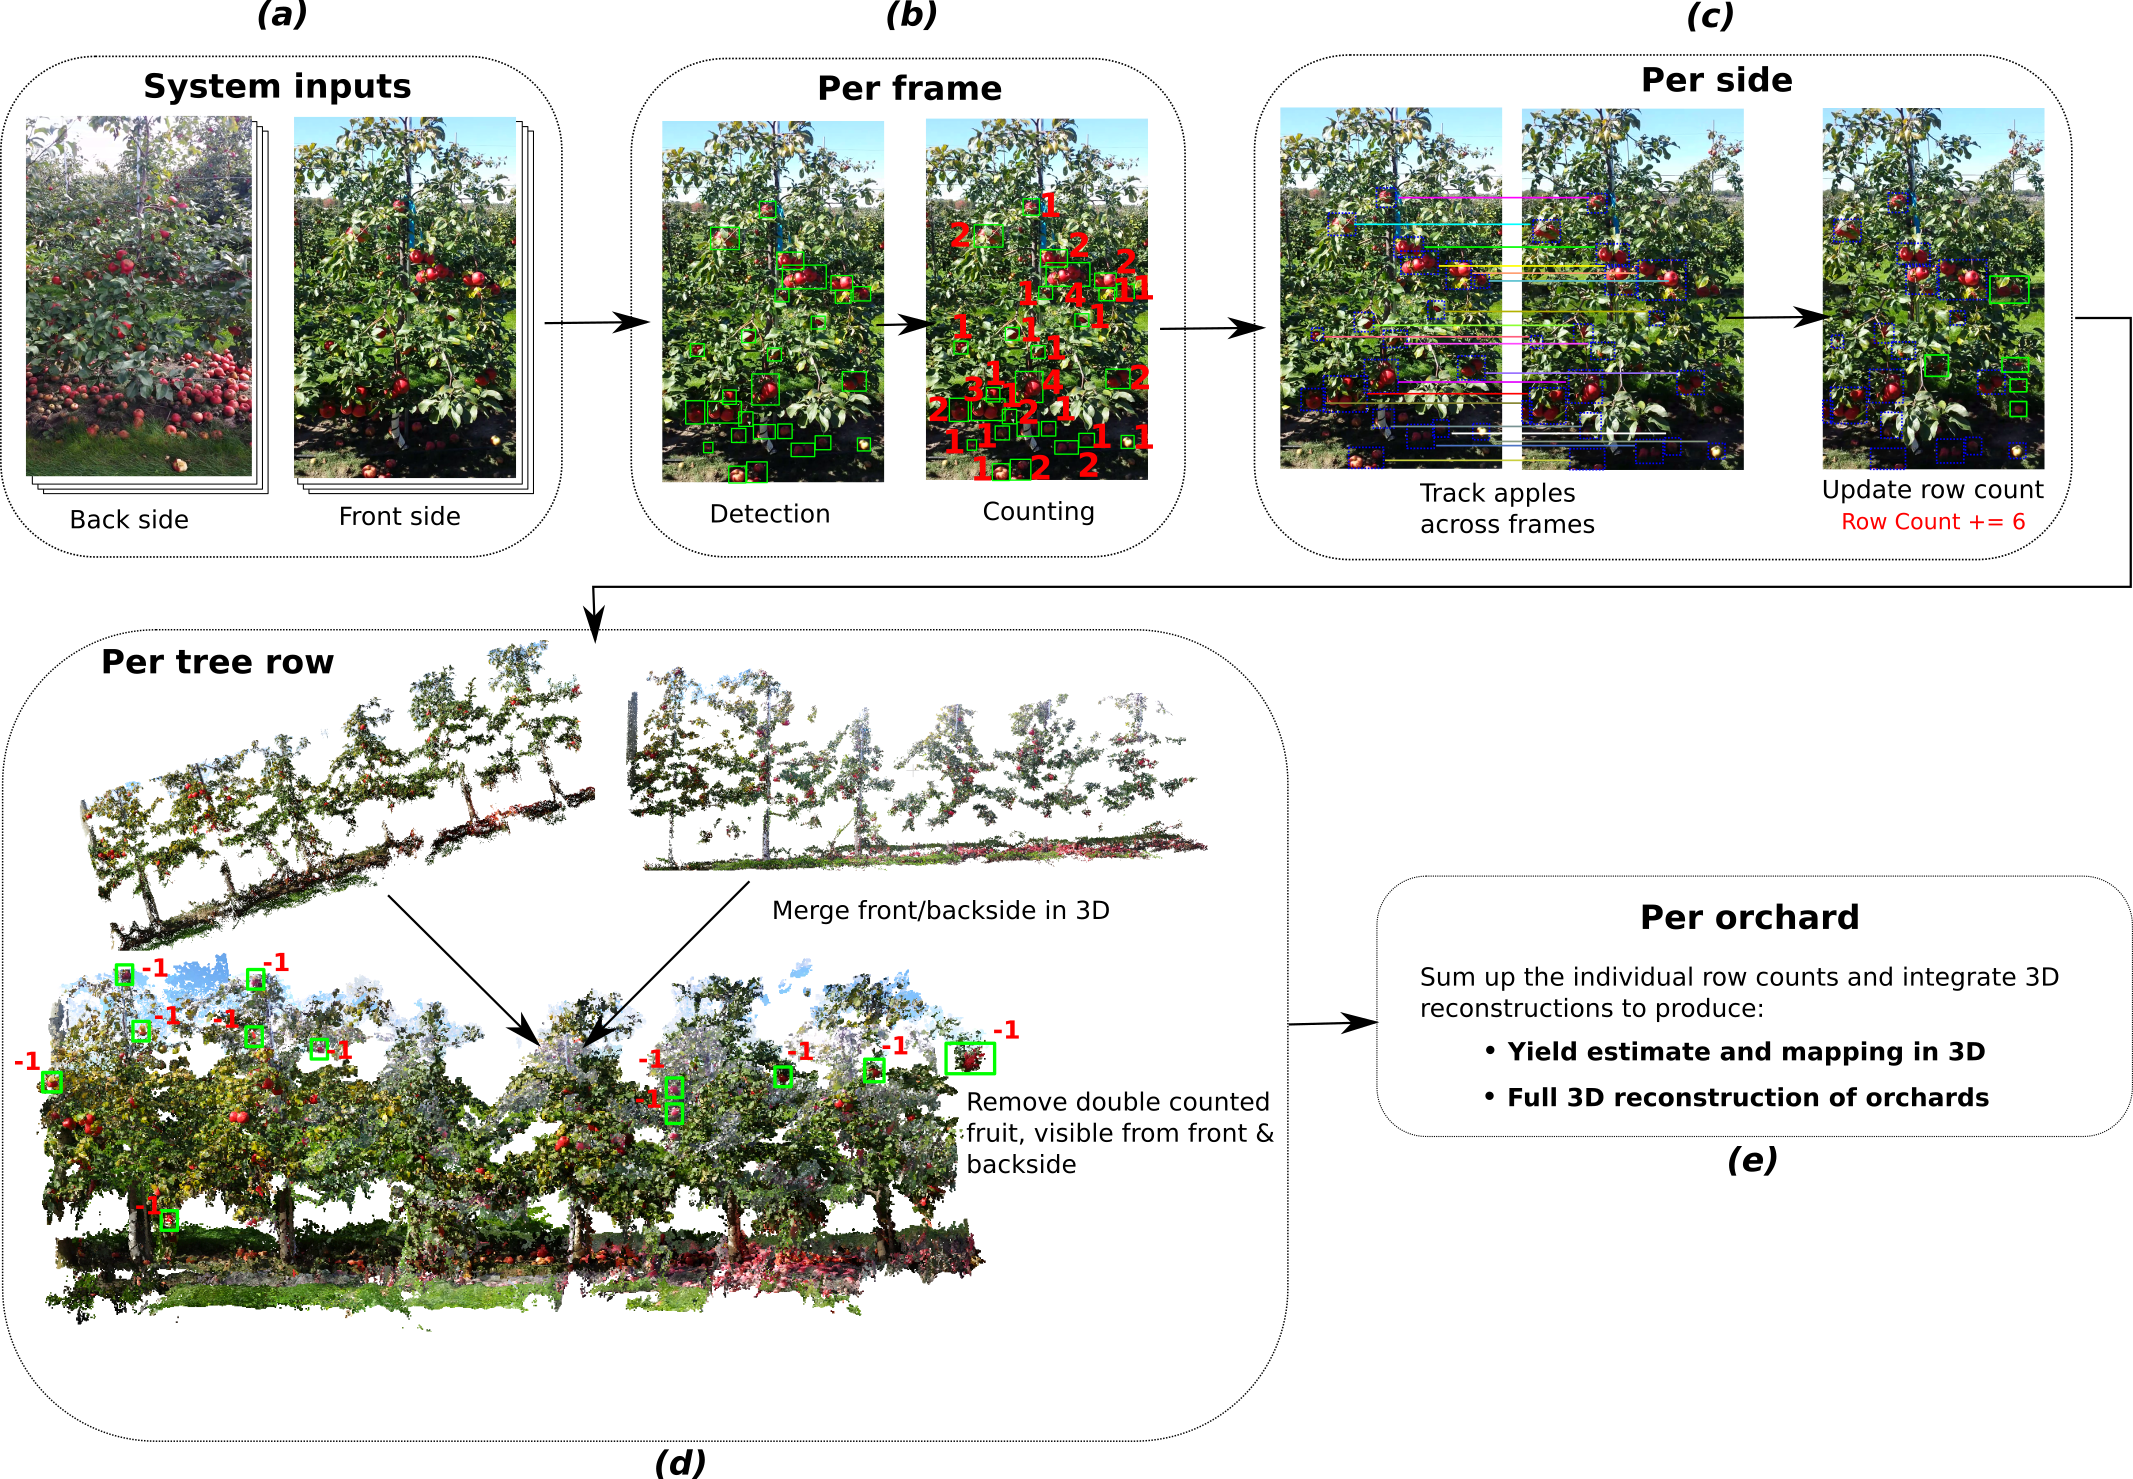
\includegraphics[width=\textwidth]{figures/prelim/conceptFigure.png}
    \caption[Overview of the yield estimation process.]{Overview of the yield estimation process. (a) Given two image sequences from the same portion of an orchard row, one from the front and one from the back. (b) fruits are detected and counted in each frame. (c) fruit are tracked across the image sequence to avoid double counting. As outputs, we have an image sequence per side, together with fruit locations and counts. (e) We reconstruct each image sequence in 3D and merge the two reconstructions into a single 3D model of the tree row. For yield estimation, we can now remove fruit visible from both sides of the tree row. (f) The pipeline produces yield estimates together with a 3D reconstruction and fruit mapping.}
    \label{fig:concept}
\end{figure*}

Second, we study the problem of realistic synthetic data generation for training deep neural networks. Deep learning solutions are general and can be applied to a wide range of problem domains. However, these solutions require a large amount of training data. Obtaining such data for many problems (e.g. fruit detection) is difficult (See Fig.~\ref{fig:labeled_instance}). Synthetic data can eliminate the painstaking problem of data annotation. As we design the models ourselves, the labeling comes for free. A network trained only on synthetic data though does not generally perform well on real data. Synthetic data differ from real data on two different levels. One, it is time-consuming and almost impossible to design synthetic data that looks identical to the real data leading to some differences in the colors and textures. This is known as the image level difference. Second, modern deep convolutional networks learn their feature descriptors from data and at the feature level, synthetic and real data can differ significantly. This is known as the feature level difference. These two difference together is defined as the domain gap. 

We present a method to reduce this domain gap in an adversarial framework. We present a method that jointly translates the synthetic images and their underlying semantics to the domain of the real data so that an adversarial discriminator (a deep neural network) cannot distinguish between the real and synthetic data. This method enables us to stylize the synthetic data to any fruit, lighting condition and environment. It can be applied to a wide variety of domain transfer tasks beyond fruit detection and counting (e.g from Grand Theft Auto (GTA)~\cite{gta} $\to$ Cityscapes~\cite{cordts_cityscapes_2016} for autonomous driving).  Additionally, it enables us to perform image to image translation with significant changes in underlying geometry (e.g from circles $\to$ triangle, sheep $\to$ giraffe, etc).


\begin{figure}[!hbpt]
{\centering
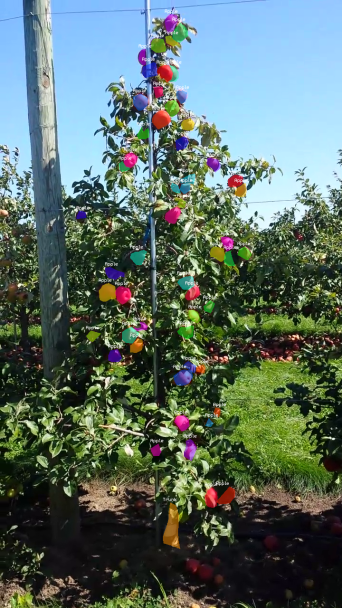
\includegraphics[width=0.25\columnwidth]{figures/prelim/instance.png}
\caption[Annotated  fruit boundaries.]{
Labeled apples. Labeling fruit boundaries precisely in images is a challenging task. Even for adept graduate students of computer vision, it takes around 20 minutes or more to label all the fruit on an average apple tree \label{fig:labeled_instance}}
}
\end{figure}


In the rest of this section, we present a high-level problem formulation, discuss specific sub-problems related to yield mapping, and other precision farming tasks and highlight our contributions.




\section{Problem Setup for Yield Mapping and Contributions }
%\label{chapter:preliminaries}

We start with a high-level problem formulation of the yield mapping problem:``Given two captured image series of the same portion of a tree row from a monocular camera (i.e. cell phone, Go-Pro etc)- one from the front side of the row and one from the backside- we want to estimate the total fruit counts and locations for the captured portion of the row.'' See Fig.~\ref{fig:concept} for an overview of the proposed system.

%

An end to end solution to this problem involves solving multiple sub-problems such as fruit detection, counting, tracking fruit across multiple views and merging fruit counts from both sides of a row. The presented system in this dissertation strives to minimize the coupling between the solutions to different sub-problems. Essentially, the design goal is to ensure that the solution to a particular sub-problem can be changed without affecting others (i.e the fruit detection methods can be changed without affecting the counting methods). 

To ensure this logical separation, we divide our system into multiple components including fruit detection, fruit counting, recovering scene geometry for tracking fruit from a single side, merging scene geometry from both sides of a row, and finally an accumulator for computing the actual yield. The proposed system detects and counts fruit in individual images, and the fruits are tracked across an image sequence using estimated camera motion and scene geometry. Afterward, independent single side reconstructions are merged into a coherent 3D model. With the assistance of this model, the system eliminates duplicate fruit counts owing to fruit visible from both sides. In addition to this complete system for yield mapping, we present an active view planning technique that can produce more precise fruit counts which is useful for phenotyping studies. Finally, we present a GAN based image to image translation technique that jointly encodes both the image and underlying semantics information and simultaneously translates them both to the target domain. Next, we provide a brief overview of all of these components.

%
\section{Fruit Detection}\label{subsec:syssegmentation}

Detecting fruit is a precursor to all the other components. The fruit detection module takes as input a color image for each frame, and outputs a binary mask which marks whether each pixel in the image belongs to the class \texttt{fruit} (Fig.~\ref{fig:detection_papers}(a)). In this dissertation, we present two different approaches to fruit detection. 

Our first approach is a semi-supervised color-based clustering technique utilizing Gaussian Mixture Models (GMM) and Expectation-Maximization (EM)~\cite{em}. In this approach, the image is over-segmented into SLIC superpixels (\cite{achanta2012slic}), using the LAB~\cite{connolly1997study} colorspace. A single representative color (mean LAB color of the pixels within the superpixel) is assigned to each superpixel. Then superpixels are clustered by color into approximately $25$ color classes. Finally, it is determined for each class whether it describes fruit, based on KL divergence (\cite{goldbergerKLdivergence}) from hand-labeled classes. These hand-labeled classes can be obtained from the unsupervised clusters of the first few frames of a particular video, to easily account for current lighting conditions and the color of the particular fruit variety at its particular ripeness (See Fig.~\ref{fig:detection_papers}(a)).


\begin{figure*}[!hbpt]
    \centering
    \includegraphics[width=\textwidth]{figures/prelim/detectionpaper.pdf}
    \caption[Developed fruit detection algorithms.]{ (a)A semi-supervised fruit detection technique based on color based clustering (b) Fruit detection using U-Net.}
    \label{fig:detection_papers}
\end{figure*}

While the semi-supervised color-based clustering technique is intuitive and simple to train, it is hard to generalize across different datasets. To resolve this problem, we present a novel approach~\cite{hani_jfr_counting} based on a deep pixel-wise segmentation network, U-Net~\cite{ronneberger_u-net:_2015}. In this approach, each pixel in the image is assigned a class (apple/background), and our objective is to minimize the total classification error. We analyze the performances of both these approaches on multiple datasets. This component is presented in detail at Chapter~\ref{chapter:detection} (See Fig.~\ref{fig:detection_papers}(b)). 

\textbf{Publications:} The results of this research appeared in two separate journal papers: Computers and Electronics in Agriculture~\cite{roy2018arxiv} and the Journal of Field Robotics~\cite{hani_jfr_counting}. 



\section{Fruit Counting}\label{subsec:sysperframecounting}
\begin{figure*}[!hbpt]
    \centering
    \def\svgwidth{\textwidth}
    \import{figures/prelim/}{countingpaper.pdf_tex}
    %\includegraphics[width=\textwidth]{figures/prelim/countingpaper.pdf}
    \caption[Developed fruit counting algorithms.]{ (a)Fruit counts for a sample fruit cluster. (b)Sample output of the shape-based clustering algorithm. These two images illustrates the difference in the number of pixels occupied by individual apples. Our algorithm works for both cases regardless of any tuning, whereas techniques such as Circular Hough Transform (CHT) need to be tuned for maximum/minimum fruit size for each case. (c)A deep ResNet-based multi-class classification approach for counting fruit. }
    \label{fig:counting_papers}
\end{figure*}

After detecting fruit, we compute the number of fruit in each of the captured frames. The counting component takes as input the binary segmented mask for each frame and outputs a set of bounding boxes and associated integers for each frame where each bounding box represents a connected cluster of fruit, and the integer is the estimated number of fruit in that cluster (See Fig.~\ref{fig:counting_papers}).

First, a connected component analysis is performed on the binary fruit mask. Each connected component is examined separately, to determine how many fruits it contains. To estimate the fruit counts accurately, we developed a method based on a classic clustering technique: Gaussian Mixture Models (GMM) (\cite{em}). Our method provides both the counts and location of individual fruit in an input image. Our method models each fruit with a Gaussian probability distribution function (pdf) and each fruit cluster with a mixture of Gaussians. Afterward, we use a novel heuristic to find the correct number of components (i.e the number of fruit) in the mixture model. Additionally, we compared this approach to one of our latter work presented in \cite{hani_apple_2018}, which poses fruit counting as a multi-class classification problem. This module is presented in detail at Chapter~\ref{chapter:fruit_counting} (See Fig.~\ref{fig:counting_papers}). 

\textbf{Publications:} The initial results of this research appeared in ISER 2016~\cite{roy2016counting} and AgriControl 2016~\cite{peng2016semantic}. Extended results and comparison with the deep learning-based approach appeared in IROS 2018~\cite{hani_apple_2018} and two previously mentioned journal versions: Computers and Electronics in Agriculture~\cite{roy2018arxiv} and the Journal of Field Robotics~\cite{hani_jfr_counting}. 



\section{Estimating Scene Geometry and Camera Motion}\label{subsec:syscammotion}

Tracking is an essential task to avoid double counting of fruit. For yield mapping, we need to track the fruit in the images captured from a single side of a tree row. Additionally, we also need to track them from the other side of the row owing to fruit visible from both sides. We develop two separate components for this task. First, we designed a method that takes the entire sequence of images from a single side of a tree row, the detected fruit clusters and their counts as input. The output is a total count of unique apples seen in the frame sequence (Fig.~\ref{fig:tracking}, \ref{fig:incsfm_intro}).

\begin{figure*}[!hbpt]
    \centering
    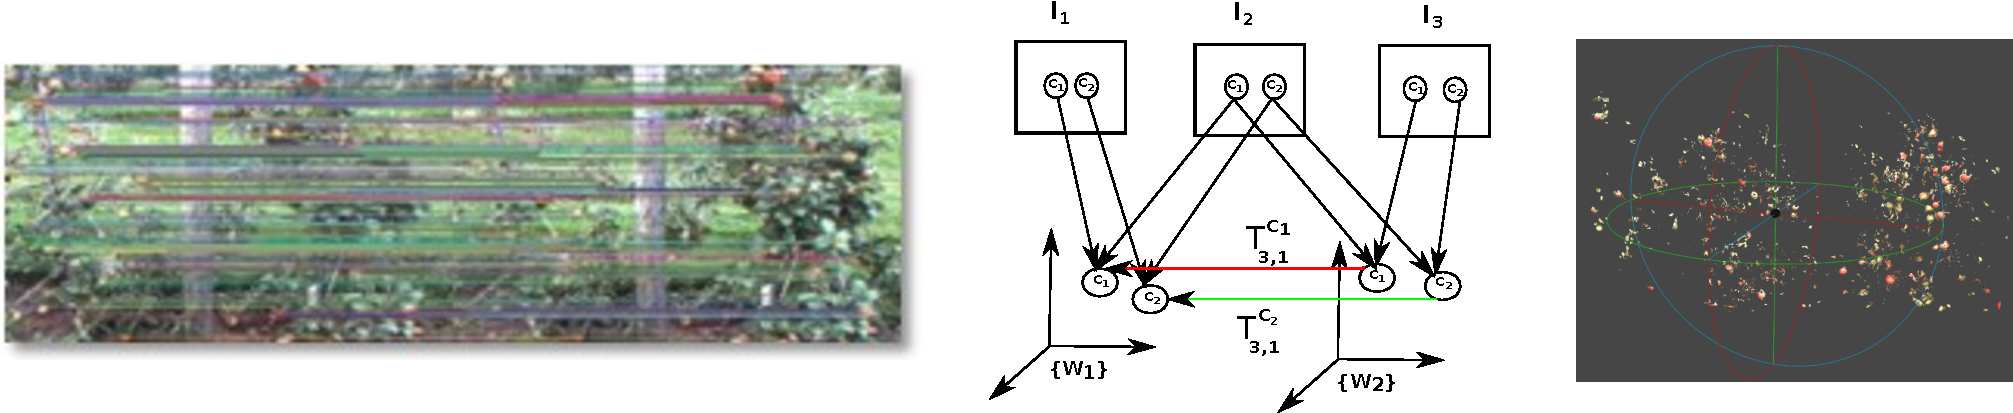
\includegraphics[width=\textwidth]{figures/prelim/case.pdf}
    \caption[Incremental structure from motion with fruit as features.]{ Incremental structure from motion with fruit as features. }
    \label{fig:incsfm_intro}
\end{figure*}

This component builds an up to scale dense reconstruction from a single side using incremental Structure from Motion (SfM)~\cite{sinha2014multi}. A standard SfM pipeline detects SIFT~\cite{surffeature} or SURF~\cite{sift} features, matches them across images and triangulates them to compute the 3D scene structure. In orchard settings though, these features are not reliable. They are often detected on the corners and edges of the leaves and branches which can move a lot in the presence of wind. This, in turn, leads to wrong matches and sparse reconstructions useless for tracking fruit and estimating fruit diameter. To resolve this problem, we developed a novel SfM pipeline where fruit contours are directly used for generating dense point matches. These matches are then used for computing the 3D scene structure and estimating camera motion. Our method operates in a sequential manner alleviating the need for computing feature matches across all the frames (the cost of feature matching is $\mathcal{O}(n^2)$ where $n$ is the number of total frames).  This component is presented in detail in Chapter~\ref{chapter:sfm}. \\

\begin{figure}[!hbpt]
{\centering
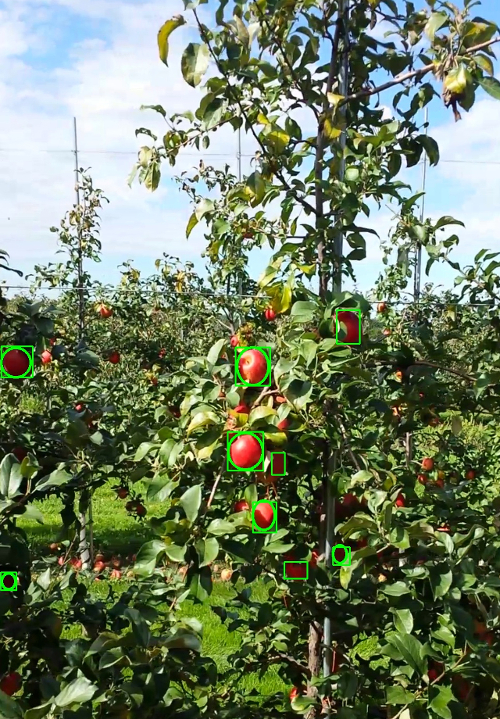
\includegraphics[width=0.3\columnwidth]{figures/prelim/tracking11.jpg}
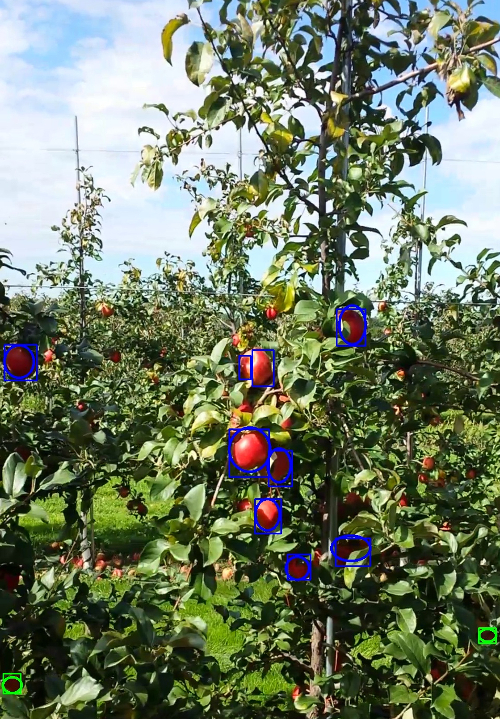
\includegraphics[width=0.3\columnwidth]{figures/prelim/tracking22.jpg}
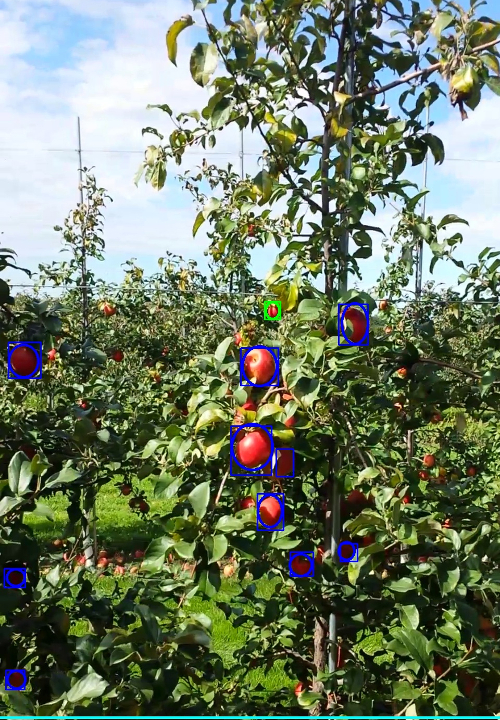
\includegraphics[width=0.3\columnwidth]{figures/prelim/tracking33.jpg}
%%%
\caption[Tracking fruit in consecutive frames]{
Tracking apples across three consecutive images. Leftmost image is the first frame. In consecutive frames, apples detected earlier are shown in blue. New apples are circled green. \label{fig:tracking}}
}
\end{figure}

\textbf{Publications:} The results of this research appeared in CASE 2016~\cite{roy2016surveying}. 

\section{Merging Scene Geometry from Both Sides}\label{subsec:sysmergecount}

To eliminate redundant fruit counts owing to fruit visible from both sides (Fig.~\ref{fig:concept} (d)), it is essential to build an accurate 3D reconstruction of the portion of the tree row under consideration. These models are also useful for automated pruning of trees and extracting geometric traits such as canopy volume, tree height, and trunk diameter.
Existing techniques such as SfM or RGB-D SLAM \cite{sturm2012benchmark,roy2016surveying} including the method described in the previous section can generate reconstructions of individual sides of the rows. However, these methods can not merge these two reconstructions. Merging the two side-reconstructions is difficult due to the lack of overlap between the two partial reconstructions. To resolve this problem, we present a novel method that utilizes global features to constrain the solution. Specifically, we use information from the silhouettes and the ground plane for alignment. This component takes the single side reconstructions as input and outputs a merged reconstructions~\cite{roy_registering_2018}. It is presented in details at Chapter~\ref{chapter:merge_both}.\\
 
\begin{figure*}[!hbpt]
    \centering
    %\def\svgwidth{\textwidth}
    %\import{figures/prelim/}{problem_goal.pdf_tex}
    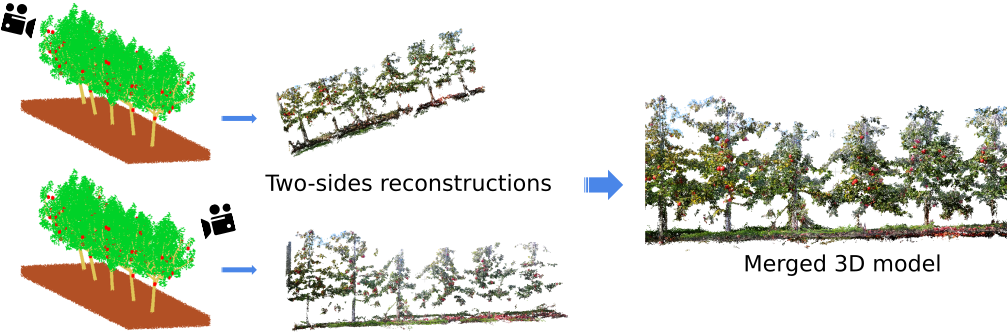
\includegraphics[width=\textwidth]{figures/prelim/problem_goal.png}
    \caption[Merging reconstructions from both sides.]{ Merging reconstructions from both sides.}
    \label{fig:fruit_yield_intro}
\end{figure*}
\textbf{Publications:} The initial results of this research first appeared in IROS 2018 ~\cite{roy_registering_2018}. An extended version appeared in the Journal of Field Robotics~\cite{dong2018semantic} .

\section{Fruit Yield Estimation}\label{sec:fruityield}
Finally, we present a component that puts everything together. It takes the fruit counts from single sides, the merged reconstructions and computes the combined fruit count for the captured portion of the tree row. It eliminates fruit on the ground and other rows and avoids double counting due to fruit visible from both sides. This is described in detail in Chapter~\ref{chapter:merge_both}. Next, we present an independent module for accurately counting fruit using active perception and a general framework for image to image translation along with underlying semantics. \\
\begin{figure*}[!hbpt]
    \centering
    \includegraphics[width=\textwidth]{figures/prelim/fruityield.pdf}
    \caption[Fruit yield estimation.]{ Fruit yield estimation}
    \label{fig:fruit_yield_full}
\end{figure*}
\textbf{Publications:} These results appeared in ISER 2016~\cite{roy2016counting} and IROS 2018 ~\cite{roy_registering_2018}. Extended versions appeared in previously mentioned journal publications~\cite{roy2018arxiv,dong2018semantic,hani_jfr_counting}.

\section{Active Fruit Counting}\label{sec:activecounting} Thus far we have presented modules that constitute a complete system for automated yield mapping where images have been captured along an arbitrary and/or predetermined path. This approach is sufficient for large commercial orchards that have ``fruit-walls" where the fruit is visible from the outside and the clusters are small. However, in more general settings, estimating the exact count from an arbitrary view is difficult. See Fig.~\ref{fig:active_counting_intro} (b). We have developed a system (Fig.~\ref{fig:active_counting_intro}(a)) that can leverage active vision techniques to accurately obtain the number of apples in a cluster. We present a method for efficiently enumerating combinatorially distinct world models (Fig.~\ref{fig:active_counting_intro}(c,d)) and computing the most likely model from one or more views. These are incorporated into single and multi-step planners. We evaluate these planners in simulation as well as with experiments on a real robot. We study this novel active perception problem in chapter~\ref{chapter:active_counting}.\\

\begin{figure*}[!hbpt]
    \centering
    \def\svgwidth{\textwidth}
    \import{figures/prelim/}{activecounting.pdf_tex}
    \caption[Active perception for counting fruit.]{ Active perception for counting fruit. Fig.~(a) shows our setup with a manipulator mounted on a ground robot. Fig.~(b) shows a challenging scenario for counting fruit from individual views. It is impossible to predict that there are six apples from any of these images individually. Fig.~(c) shows combinatorial world models for a fruit cluster with three apples and models which are combinatorially redundant. }
    \label{fig:active_counting_intro}
\end{figure*}

\textbf{Publications:} The results of this research appeared in IROS 2017~\cite{roy2017active}.

\section{Semantics-aware image to image translation and domain transfer}
For many precision farming and phenotyping tasks such as fruit detection and counting, deep learning solutions are very effective and can be translated easily to other specialty crops. Such solutions though require a lot of labeled data and annotating such data precisely is tedious and cumbersome. To eliminate the painstaking process of data annotation, we present a framework for realistic synthetic data generation using image to image translation.
Image to image translation is the problem of transferring an image from a source to a target domain. State-of-the-art methods fail in the presence of significant geometric changes between the two domains. These failures can be attributed to the inability of translating methods to learn the underlying semantics of the images. To solve this problem, we present a method based on Generative Adversarial Networks (GAN) that can leverage underlying semantic information. We develop an encoder-decoder based generator architecture that jointly encodes both the image and underlying semantics information and simultaneously translates them both to the target domain. Additionally, for object transfiguration and domain transfer tasks, we propose additional loss terms that encourage preserving the background underlying semantics. This component is presented in detail at chapter~\ref{chapter:semgan}(See Fig.~\ref{fig:intro_sem}).\\

\begin{figure*}[!htbp]
    \centering
    \def\svgwidth{\textwidth}
    \import{figures/prelim/}{intro_thesis.pdf_tex}
    \caption[Semantics-aware image to image translation and domain transfer]{Given two unpaired image collections and semantic label masks, our network learns a mapping to translate images from one domain to the other while preserving the labels. Top left: Object transfiguration task for circles to triangles. Top right: Image to image style transfer from Horses to Zebras. Bottom: Domain translation from synthetic GTA to Cityscapes photos. The examples show the CycleGAN~\cite{zhu_unpaired_2017} output, the image and mask outputs of our method. Note that CycleGAN does not output masks.}
    \label{fig:intro_sem}
\end{figure*}

\textbf{Publications:} A journal paper is currently under preparation~\cite{roy2019_semgan}.\\


With the problem formulation and different sub-problems of interest clearly stated, we are now ready to position this dissertation with respect to the existing literature.

